% !TEX root = ../thesis-example.tex
%
%************************************************
% Kern der Arbeit
%************************************************
\chapter{Reranking mittels Click-Trough-Rate Ergebnis}
\label{sec:Reranking}

%Prozessaufbau des Lösungsansatzes
%----------------------------------------------------------------

\section{Prozessaufbau des Lösungsansatzes}
\label{sec:Reranking:Prozessaufbau}

\subsection{Prozessaufbau als Bild}
\label{sec:Reranking:Prozessaufbau:ProzessaufbauBild}

\begin{figure}[H]
\centering
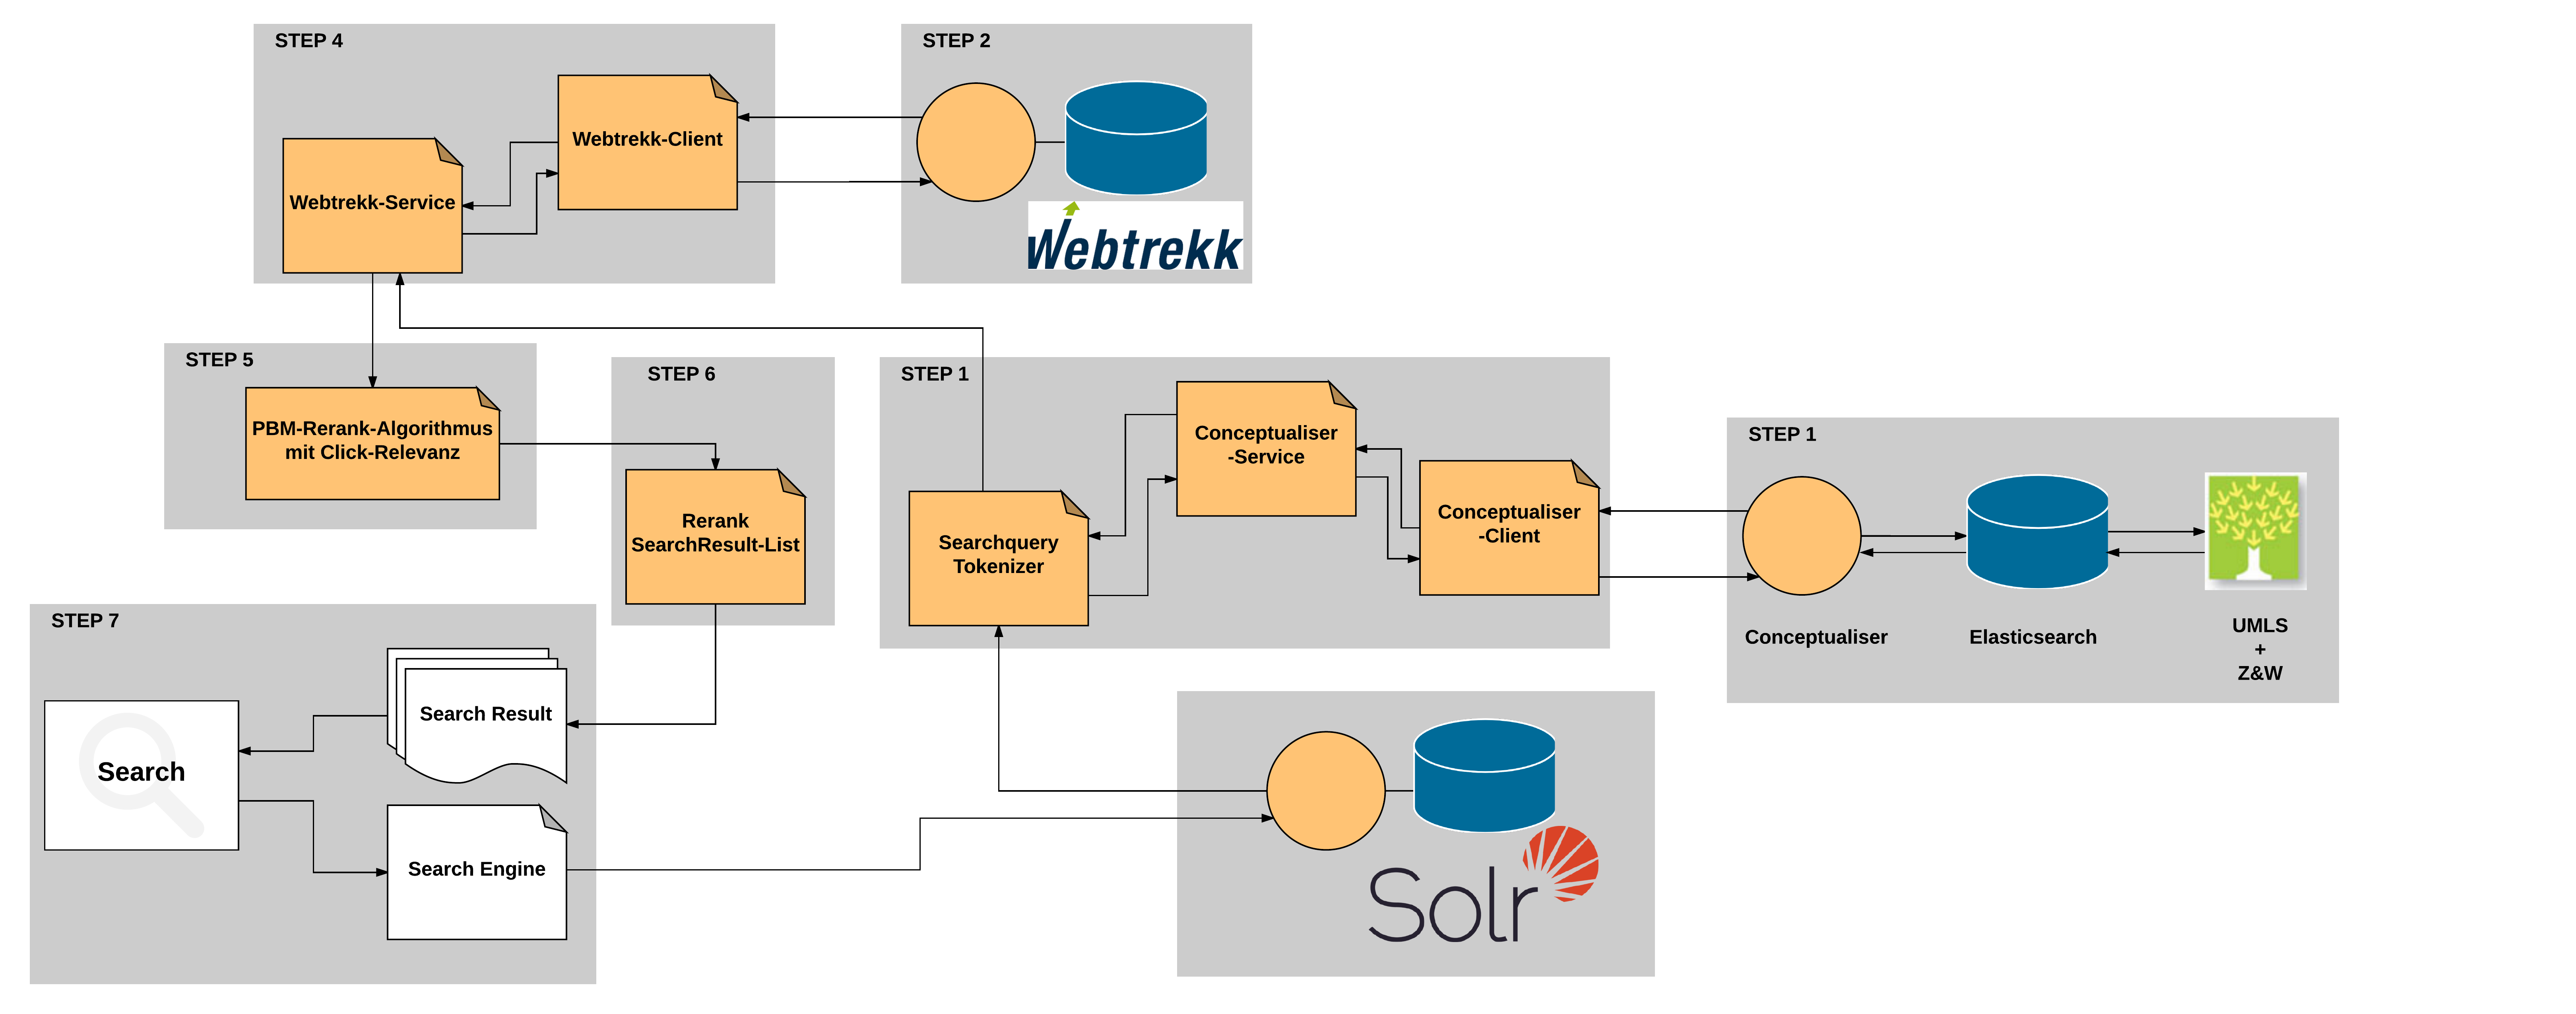
\includegraphics[width=0.5\linewidth]{gfx/Prozessaufbau}
\caption[Prozessaufbau des Lösungsansatzes]{Prozessaufbau des Lösungsansatzes}
\label{fig:Prozessaufbau}
\vspace{-2.5em}
\end{figure}

\subsection{Probleme des Lösungsansatzes}
\label{sec:Reranking:Prozessaufbau}

\subsection{Suchterm Segmentierung}
\label{sec:Reranking:Prozessaufbau:SuchtermSegmentierung}

\subsection{Aufbereitung Click-Trough-Daten}
\label{sec:Reranking:Prozessaufbau:Click-Trough-Daten}

\subsubsection{Kein Einfluss auf Suchergebnisqualität während der Klicks}
\label{sec:Reranking:Prozessaufbau:Click-Trough-Daten:Click-Trough-Suchergebnisqualität}

siehe Grundlagen

\subsubsection{Userverhalten}
\label{sec:Reranking:Prozessaufbau:Click-Trough-Daten:Click-Trough-Userverhalten}

Die Webtrekk-Analysen bieten uns nur beschränkte Informationen zum Klick-Verhalten der User. Wichtige Informationen wie die Verweildauer auf einem Dokument oder ob nach diesem Dokument ein weiteres Dokument zum gleichen Suchterm angeklickt worden ist, lassen diese Analysen nicht zu. 

\subsection{Click-Trough-Rate in Suchprozess einbinden}
\label{sec:Reranking:Prozessaufbau:SucheEinbinden}

- Solr gebundene Suchresultatmenge
- Pagination (Einfluss von Reranking)

\subsection{Result-Reranking mittels PBM Algorithmus}
\label{sec:Reranking:Prozessaufbau:Result-RerankingPBM}

- Smoothing

- Mehrfachverwertung von Content 
	=> mehrfache Auflistung in Suchergebnissen (nicht Teil dieser Arbeit)
- Algorithmus nicht festfahren (Overfitting)

- User nicht festfahren auf altem Wissen 
	- aktuelle und neue Publikationen werden nicht berücksichtigt 
		=> keine Userrelevanz (nicht Teil dieser Arbeit)
		
%Methodik
%----------------------------------------------------------------

\section{Methodik}
\label{sec:Reranking:Methodik}

In Kapitel \ref{sec:Grundlagen:Grundbegriffe} haben wir gelernt wie Click-Trough-Daten entstehen und wie sie zu lesen sind. Nun können wir mit diesem Wissen die Click-Trough-Rate der Dokumente berechnen. Mithilfe der berechneten Click-Trough-Daten werden wir dann ein \textit{Reranking} der Suchresultate durchführen. So wollen wir die Userrelevanz in die Suche einbinden. Die Vorgehensweise dazu sieht wie folgt aus.

\subsection{Suchterm Segmentierung}
\label{sec:Reranking:Methodik:SuchtermSegmentierung}

\subsubsection{Suchterm semantisch aufschlüsseln mittels Segmentierung}
\label{sec:Reranking:Methodik:SuchtermSegmentierung:SuchtermSegmentierung}

Um alle relevanten Click-Trough-Daten lesen zu können, müssen wir zunächst den Suchterm auftrennen, wie in Kapitel \ref{sec:Grundlagen:SemantikUserInteraktionen:ProblemstellungenClick-Trough-Daten} angesprochen. Die Auftrennung des Suchterms in die einzelne Worte können wir mithilfe einer Segmentierung\footnote{Bezeichnet die Aufteilung in Abschnitte, in diesem Fall in einzelne Worte} durchführen. Hier könnten wir uns überlegen, zusätzlich mit Stoppwörtern\footnote{Stoppwörter sind Wörter, die sehr häufig auftreten und für gewöhnlich keine Relevanz für den Dokumentinhalt besitzen} nicht relevante Wörter aus dem Suchterm zu entfernen. Dieses Verfahren macht aber im Springermedizin-Kontext keinen Sinn. Wie in Kapitel \ref{sec:Einfuehrung:Problemstellung:Userrelevanz} angesprochen, suchen die User der Springermedizin-Applikation oft mit einschlägig, fundierten Fachbegriffen. Wir gehen darum davon aus, dass alle Wörter des verwendeten Suchterms für das Suchergebnis relevant sind. Diese Erkenntnis basiert auf Aussagen der Redakteure von Springermedizin und Webtrekk-Analysen der meist gesuchtesten Suchtermen der letzten Monate. Auch sind Stoppwörter veraltet und werden in modernen Information Retrieval Verfahren nicht mehr eingesetzt. Wir verzichten darum auf den Einstatz von Stoppwörtern.

\subsubsection{Suchterm semantisch erweitern mittels Thesaurus}
\label{sec:Reranking:Methodik:SuchtermSegmentierung:SuchtermThesaurus}

Wie in Kapitel \ref{sec:Grundlagen:SemantikUserInteraktionen:ProblemstellungenClick-Trough-Daten} thematisiert, wollen wir die Click-Trough-Daten zu unserem Suchterm um Click-Trough-Daten zu verwandten Begriffen erweitern. Für diese semantische Erweiterung eines Suchwortes werden wir einen Thesaurus verwenden. Die Erweiterung umfasst zum Suchterm gleichbedeutende Begriffe (Synonyme), sehr ähnliche Begriffe (Narrow Terms), ähnliche Begriffe im weiteren Sinne (Broader Terms) und verwandte Begriffe (Related Terms).
\\
\\
Springer Nature besitzt einen Webservice mit welchem auf den Thesaurus \textit{Unified Medical Language System} (UMLS)~(siehe \cite{UMLS}) zugegriffen werden kann. Der Webservice nimmt einzelne Wörter und Wort-Listen entgegen. Zu jedem dieser Wörter durchsucht der Webservice den Thesaurus nach den oben erwähnten Arten von verwandten Begriffen. Der Webservice verwendet für diese Suche eine Elasticsearch~(siehe \cite{elasticsearch})\footnote{Eine Elasticsearch ist eine Volltextsuchmaschine}. Die dabei gefundenen Begriffe, liefert der Webservice als Antwort zurück. Um alle relevanten Click-Trough-Daten zu finden, werden wir mit dem segmentierten Suchterm eine Anfrage gegen diesen Webservice stellen und anschließend den segmentierten Suchterm um die gefundenen Begriffe erweitern. Mithilfe des erweiterten Suchterms können wir dann anschließend eine Analyse in Webtrekk starten und alle relevanten Click-Trough-Daten lesen. 

\subsection{Aufbereitung Click-Trough-Daten}
\label{sec:Reranking:Methodik:Click-Trough-Daten}

\subsubsection{Jeder Klick auf ein Dokument ist relevant}
\label{sec:Reranking:Methodik:Click-Trough-Daten:Click-Trough-DatenAuswertungen}

Wie in Kapitel \ref{sec:Reranking:Grundlagen:Click-Trough-Daten:UserverhaltensFeedback} beschrieben, reichen Webtrekk-Analysen für komplexe Auswertungen der Click-Trough-Daten nicht aus. Wir können darum in dieser Arbeit \textit{Feedback-Strategien} für die Click-Trough-Rate Auswertung, wie in \cite{Joachims} beschrieben, nicht verwenden. Stattdessen greifen wir wie ebenfalls in Kapitel \ref{sec:Reranking:Grundlagen:Click-Trough-Daten:UserverhaltensFeedback} beschrieben auf die Click-Trough Features zu, die uns Webtrekk zur Verfügung stellt. Daraus entsteht ein interpretierbares Feature-Set. Dieses ist leider sehr klein und enthält keine Informationen um ein Relevanzfeedback zu den Klick-Häufigkeiten daraus lesen zu können. Wir müssen wir darum davon ausgehen, dass jeder Klick auf ein Dokument relevant ist.

\subsubsection{Gewichtung der Click-Trough-Daten}
\label{sec:Reranking:Methodik:Click-Trough-Daten:Gewichtung}

Durch die semantische Aufschlüsselung des Suchterms haben wir verschieden starke Relationen zwischen Click-Trough-Daten und dem Suchterm. Die Gewichtung der Stärke dieser Relation ist aber nicht Kern dieser Arbeit. Wir gehen darum davon aus, dass unabhängig der stärke der Relation zum Suchterm, alle Click-Trough-Daten eine gleiche Relevanz besitzen.

\subsubsection{Berechnung der Click-Trough-Rate}
\label{sec:Reranking:Methodik:Click-Trough-Daten:Gewichtung}

Die Click-Trough-Rate wird vor allem im Bereich des Internet-Marketing verwendet und stellt grundsätzlich die Anzahl der Klicks auf ein Dokument oder Link im Verhältnis zu den gesamten Impressionen dar. Bezogen auf das in Kapitel \ref{sec:Reranking:Grundlagen:Click-Trough-Daten:UserverhaltensFeedback} angesprochene Feature-Set, würden die \textit{ClickProbability}~(Klick-Wahrscheinlichkeit) direkt als Click-Trough-Rate verwenden. Dazu müssten wir nur die Click-Trough-Daten eines Dokuments ins Verhältnis zu allen Click-Trough-Daten für einer Suchanfrage stellen. Wie wir aber bereits in Kapitel \ref{sec:Grundlagen:SemantikUserInteraktionen} gelernt haben, würden wir damit viele Problemstellungen der Interaktion der User mit der Suche ignorieren. Deswegen verwenden wir den Position-Based Modell basierten Algorithmus um mithilfe dieses angesprochenen Feature-Sets die Click-Trough-Rate zu berechnen.

\subsection{Result-Reranking mittels PBM basiertem Algorithmus}
\label{sec:Reranking:Methodik:Result-RerankingPBM}

\subsubsection{Klick-Wahrscheinlichkeit mit Position-based Modell berechnen}
\label{sec:Reranking:Methodik:Result-RerankingPBM:Klick-Wahrscheinlichkeit}

Wie in Kapitel \ref{sec:Grundlagen:Grundbegriffe:Result-RerankingPBM:AnsatzSucheEinbinden} angesprochen, werden wir unseren Reranking-Algorithmus in die Aufbereitung der Suchresultate aus der Solr-Suche integrieren.
\\
\\
Dieser soll die Suchergebnisliste analysieren, die Click-Trough-Rate der Dokumente berechnen und die Liste neu sortieren. 
\\
\\
Wir müssen jedoch beachten, dass die Solr durch die Pagination-Funktion~(siehe \cite{Pagination}) nur die Top-N-Ergebnisse (bei Springermedizin sind es 20 Ergebnisse) zurückgibt. Dadurch sehen wir nur einen Teil der Suchergebnisse. 
\\
\\
Diese Logik liegt in der Springermedizin-Applikation im Aufbau der Suchanfrage. Daher können wir diese selber steuern und uns statt 20 beispielsweise die nächsten 100 Ergebnisse zurückgeben lassen. Am Ende filtern wir die ersten 20 Ergebnisse und stellen diese dar. Außerdem wissen wir bei diesem Lösungsansatz, in welcher Reihenfolge die Ergebnisse aus der Solr zurückgegeben werden. Wir kennen die Dokumente und deren Rang. Dadurch haben wir hilfreiches Zusatzwissen, welches wir in den Klick-Modell basierten Algorithmus einfließen lassen können.

\subsubsection{Verhältnis zwischen den Klick-Wahrscheinlichkeiten abhängig der Position im Suchresultat definieren}
\label{sec:Reranking:Methodik:Result-RerankingPBM:VerhaeltnisKlick-Wahrscheinlichkeiten}

Aus eigener Erfahrung wissen wir, dass die ersten Dokumente im Suchresultat immer zuerst gesehen werden. Die dahinter gelisteten Dokumente werden fortlaufend analysiert. Dies bestätigt die in Abb. \ref{fig:Grundlage:AnalyseKlicksPositionen} dargestellte Analyse der Klicks auf die ersten 20 Positionen eines Suchergebnisses. Wir sollten darum darauf achten, dass je \textit{schlechter} der Rang des angeklickten Dokumentes im Suchresultat der Solr ist, desto \textit{höher} das Relevanzfeedback zu bewerten ist. 
\\
\\
Das machen wir, indem wir für die Berechnung der Click-Trough-Rate das Verhältnis zwischen Klick-Wahrscheinlichkeit der Position und Klick-Wahrscheinlichkeit des Dokumentes abhängig der Position im Suchresultat definieren. Als Grundlage hierbei dient uns die Position des Suchresultats der Solr. In der folgenden Tabelle sehen wir die Aufteilung der Verhältnisse abhängig der Position:

\begin{table}[H]
\centering
\begin{tabular}{|c|c|c|}\hline
	\textbf{Position} & \textbf{Verhältnis Position zu Dokument}\\ \hline
	1 bis 10 & 1:1 \\ \hline
	11 bis 20 & 1:2 \\ \hline
	größer 20 &  1:3 \\ \hline
 \end{tabular}
 \vspace{.5em}
 \caption[Verhältnis Klick-Wahrscheinlichkeiten der Position zu der des Dokumentes]{Verhältnis Klick-Wahrscheinlichkeiten der Position zu der des Dokumentes}
\label{tab:VerhaeltnisKlick-WahrscheinlichkeitenPositionDokument}
\vspace{-2.5em}
\end{table}

Für die Suchresultate mit einer Position über 20, verstärken wir die Gewichtung der Klick-Wahrscheinlichkeit des Dokumentes erheblich. Das liegt daran, dass bei Klicks auf Dokumente mit einer solch hohen Position wir davon ausgehen können, dass die suchende Person die Suchresultate genau analysiert hat, bevor sie ein Dokument angeklickt hat. Haben wir die Verhältnisse definiert, müssen wir diese in den Algorithmus einbauen. Wie wir dies machen, werden wir im folgenden Abschnitt anschauen.

\subsubsection{Smoothing Faktor in Position-based Modell}
\label{sec:Reranking:Methodik:Result-RerankingPBM:SmoothingPBM}

Wir wissen dass eine Wahrscheinlichkeit einen Wert zwischen 1 und 0 besitzt. Dadurch können Nullwerte entstehen. Das PBM multipliziert die Positions- und Dokument-Wahrscheinlichkeit miteinander, um die Klick-Wahrscheinlichkeit zu berechnen. Wir müssen aber davon ausgehen, dass es Dokumente geben kann, deren Rang nie angeklickt worden ist und umgekehrt. 
\\
\\
Multiplikationen mit Null ergeben immer einen Nullwert. An dieser Stelle führen wir einen \textit{Smoothing-Faktor} ein. Der Smoothing-Faktor soll zwei Probleme lösen. Zum einen wollen wir einen Wahrscheinlichkeitswert trotz der Multiplikation mit Null beachten. Zum anderen wollen wir die im vorherigen Absatz beschriebene Gewichtung abhängig des Relevanzfeedbacks in den Algorithmus einbeziehen. Wir transformieren dazu das Produkt der beiden Wahrscheinlichkeiten in eine gewichtete Summe, dem sogenannten \textit{Weighted Moving Average}~(siehe \cite{weightedAVG}), dessen Gewichte sich zu Eins aufsummieren. Diese Gewichte sind die Smoothing-Faktoren, weshalb das Verfahren zählt zu den Smoothing-Algorithmen zählt.

\subsection{Vergessen der alten Daten}
\label{sec:Reranking:Methodik:Vergessen}

Ein Algorithmus zur Berechnung von Wahrscheinlichkeiten muss sich ein gewisses Grundwissen aneignen. Dies geschieht üblicherweise durch Trainingsdaten. Genauso muss er alte Daten wieder vergessen können, um Overfitting\footnote{Überanpassung des Algorithmus durch zu viele (falsche oder veraltete) Daten} zu vermeiden. 

\subsubsection{Durch Webtrekk ist kein komplexer Lern-Algorithmus notwendig}
\label{sec:Reranking:Methodik:Vergessen:Lern-Algorithmus}

Durch Webtrekk haben wir eine Wissensbasis, die sich stetig und zeitnah aktualisiert. So muss der Algorithmus nicht stetig neues Wissen lernen und altes vergessen, sondern er kann direkt diese Wissensbasis zugreifen. Dies geschieht, indem zur Laufzeit\footnote{Unter Laufzeit wird in diesem Fall der Zeitpunkt der direkte Abfrage während der Suchanfrage bezeichnet} Analysen gegen Webtrekk über eine frei definierbare Periode gemacht werden. Dadurch kann \textit{Overfitting} vermieden werden. Deshalb verwenden wir keinen komplexen Lern-Algorithmen wie in \cite{IWUSBI} vorgestellt.

\subsubsection{Die Klick-Wahrscheinlichkeit ist kein absoluter Wert für die Userrelevanz}
\label{sec:Reranking:Methodik:Vergessen:Relevanzfeedback}

Nun könnten wir die Klick-Wahrscheinlichkeit als absoluten Wert für die \textit{Userrelevanz} betrachten. Dies wäre jedoch falsch, wie in Kapitel \ref{sec:Grundlagen:SemantikUserInteraktionen:RankExamination} analysiert, müssen wir davon ausgehen, dass viele User der Qualität der Suchmaschine vertrauen. Diese betrachten die Top-Suchresultate als die relevanten Suchresultate. Denkbar wäre auch, dass User unabsichtlich das falsche Dokument anklicken und dadurch die Click-Trough-Rate eines Dokumentes verfälschen. Dadurch kann ein \textit{Overfitting} des Algorithmus entstehen.

\subsubsection{Overfitting vermeiden}
\label{sec:Reranking:Methodik:Vergessen:Overfitting}

Um ein Overfitting zu vermeiden, darf der Algorithmus nicht immer anschlagen. Wir müssen sicherstellen, dass vereinzelt zufällige Dokumente in den \glqq Top-Suchresultaten\grqq{} angezeigt werden. So können auch andere Dokumente in den Fokus des Users gerückt werden. Das System fährt sich dadurch nicht auf falschen Annotationen fest. 

\subsubsection{Zusätzliche Varianz durch Zufallsfaktor}
\label{sec:Reranking:Methodik:Vergessen:Zufallsfaktor}

Mithilfe eines Zufallsfaktors kann eine solche Varianz in den Klick-Modell basierten Algorithmus gebracht werden. Wie bereits weiter oben erwähnt, werden viele Suchresultate nie und deren Rang selten bis gar nicht angeklickt. Sie haben darum keine Click-Trough-Daten. Deren Klick-Wahrscheinlichkeit ist entweder Null oder sehr klein. Der Zufallsfaktor soll darum nur leichte Einflüsse in die Klick-Wahrscheinlichkeitsberechnung haben. Auch hier können wir wieder mit dem oben eingeführten \textit{Weighted Moving Average} arbeiten.

%Der PBM-Algorithmus
%----------------------------------------------------------------

\section{Der PBM-Algorithmus}
\label{sec:Reranking:PBM-Algorithmus}


%Zusammenfassung
%----------------------------------------------------------------

\section{Zusammenfassung}
\label{sec:Reranking:Zusammenfassung}

